\chapter{Metrici și experimente}\label{chap:metrici}
\indent\par
Capitolul de față prezintă evaluarea experimentală a sistemului IORA, urmărind să cuantifice performanța fiecărei etape a fluxului de procesare, dar și a întregului lanț de recunoaștere. Mai întâi sunt descrise seturile de date utilizate, atât cel destinat evaluării \textit{end-to-end} a sistemului, cât și cel folosit pentru antrenarea clasificatorului de caractere, împreună cu procedeele de normalizare, adnotare și augmentare aplicate acestora. În continuare sunt introduse metricile de evaluare și sunt raportate rezultatele obținute, mai întâi pentru componenta de recunoaștere a caracterelor considerată izolat, apoi pentru sistem la nivel de etapă și \textit{end-to-end}. În final, secțiunea de experimente justifică, prin rezultate cantitative, principalele decizii de proiectare adoptate în fluxul de procesare și evidențiază contribuția fiecărei intervenții la performanța de ansamblu.

\section{Seturi de date}
\indent\par
Sistemul IORA operează cu două seturi de date distincte: un set de evaluare, utilizat pentru măsurarea performanței \textit{end-to-end} a fluxului de procesare, și un set de antrenare, destinat construirii clasificatorului SVM. Ambele gravitează în jurul aceluiași corpus de imagini cu plăcuțe de înmatriculare obținut prin platforma Roboflow~\cite{roboflow-lp-dataset}, completat, în cazul setului de evaluare, de o componentă românească colectată manual, iar în cazul setului de antrenare, de un set de date dedicat caracterelor individuale cu fonturi variate.

\subsection{Setul de evaluare}
\indent\par
Pentru a determina robustețea sistemului și capacitatea sa de adaptare la diverse formate ale numărului de înmatriculare a fost necesară crearea unui set de date mixt, în care sunt prezente atât autovehicule de pe teritoriul României, cât și vehicule din alte regiuni ale globului. Pentru prima componentă a setului de date în momentul de față nu există o sursă general valabilă și deschisă publicului larg, așadar imaginile reprezentative acestei părți au fost colectate manual de pe platforme de comerț auto online. Această procedură de salvare și utilizare a imaginilor este conformă cu reglementările GDPR, întrucât fotografiile au fost publicate în mod voluntar de către vânzători pe platforme cu acces liber, fiind astfel destinate publicului larg, iar prelucrarea lor s-a realizat strict în scop de cercetare și evaluare a sistemului. Pentru componenta internațională, a fost utilizat setul de date public obținut prin intermediul platformei Roboflow~\cite{roboflow-lp-dataset}.

\subsubsection{Normalizarea seturilor de date}
\indent\par
În contextul sistemelor de recunoaștere automată a numerelor de înmatriculare puse în funcțiune în cadrul parcărilor condițiile de execuție precum poziția numărului de înmatriculare, distanța și raportul dimensiunilor, unghiul de captare și distanța focală sunt bine cunoscute, permitând valorificarea lor în procesul de localizare.

Pentru a reproduce aceste condiții, a fost necesară normalizarea setului de date. În cazul imaginilor obținute în mod manual, acest procedeu a presupus selectarea autovehiculelor care prezentau un număr de înmatriculare vizibil, urmată de o decupare pentru a reduce zgomotul de fundal și a oferi o distanță focală relativ constantă. Un exemplu al procesului poate fi observat în figura~\ref{fig:normalizare_imagine_ro}, unde înainte de normalizare erau prezente elemente de zgomot agresive atât în parbrizul mașinii cât și în spațiul înconjurător.
\begin{figure}[H]
  \centering
  \begin{subfigure}[b]{0.45\textwidth}
    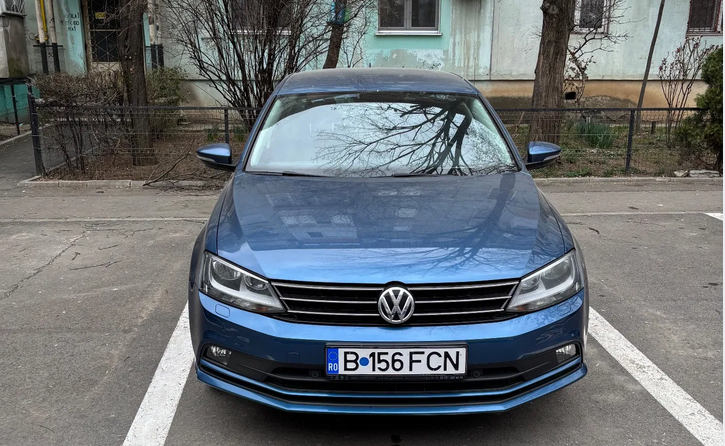
\includegraphics[width=\textwidth]{figures/b156fcn_initial.png}
    \caption{Înainte de normalizare}
    \label{fig:img_initiala}
  \end{subfigure}
  \hfill
  \begin{subfigure}[b]{0.45\textwidth}
    \includegraphics[width=\textwidth]{figures/b156fcn_cropped.png}
    \caption{După normalizare}
    \label{fig:img_decupata}
  \end{subfigure}
  \caption{Un exemplu de imagine alterată pentru a reduce zgomotul de fundal și normaliza unghiul de captură}
  \label{fig:normalizare_imagine_ro}
\end{figure}

Pentru componenta internațională a setului de date procesul a fost unul mai rapid, fiind necesară doar selectarea imaginilor corespunzătoare criteriilor menționate anterior. În figura~\ref{fig:normalizare_imagine_thl} se poate observa un exemplu de imagine corespunzătoare pusă în paralel cu o imagine care nu adera la standardele impuse.
\begin{figure}[H]
  \centering
  \begin{subfigure}[b]{0.45\textwidth}
    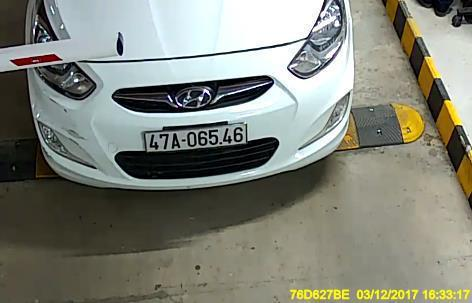
\includegraphics[width=\textwidth]{figures/imagine_buna_thl.jpg}
    \caption{Imagine corespunzătoare}
  \end{subfigure}
  \hfill
  \begin{subfigure}[b]{0.45\textwidth}
    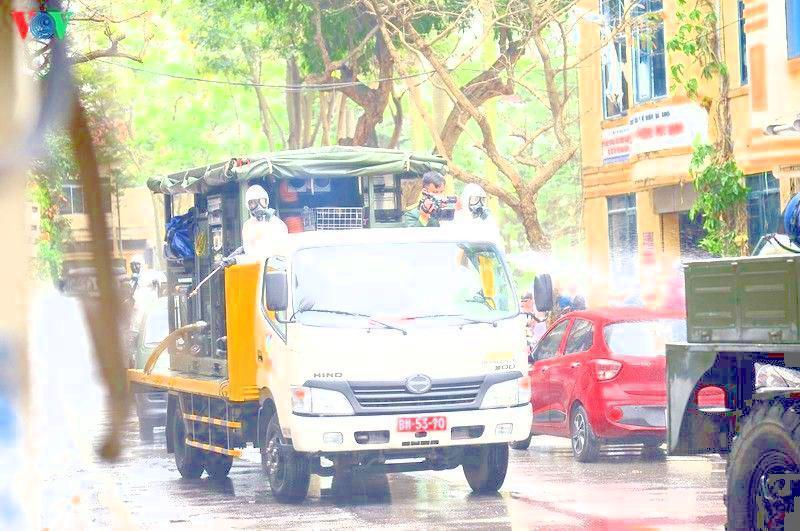
\includegraphics[width=\textwidth]{figures/imagine_proasta_thl.jpg}
    \caption{Imagine necorespunzătoare}
  \end{subfigure}
  \caption{Paralelă între o imagine conformă și una neconformă}
  \label{fig:normalizare_imagine_thl}
\end{figure}

\subsubsection{Crearea sursei de adevăr a setului de date}
\indent\par
Procedeul descris anterior constituie, însă, doar primul pas în construirea unui set de date potrivit strategiei de procesare propuse de această teză. Este în continuare necesară o sursă de adevăr uniformă pe componentele locală și internațională. Această secțiune prezintă pașii luați în completarea imaginilor cu informații relevante și conforme cu realitatea, care să reprezinte reperul față de care vor fi evaluate predicțiile generate de \textit{pipeline}.

Prima etapă este reprezentată de adnotarea imaginilor cu numărul de înmatriculare afișat în acestea, sarcină realizată manual, prin deschiderea lor rând pe rând, urmată de adăugarea valorilor într-un fișier \texttt{.csv} dedicat. Pentru a permite analizarea performanței componentei de localizare, a fost dezvoltat un utilitar \textit{software} dedicat extragerii chenarelor ce încadrează numerele de înmatriculare (\textit{bounding boxes}). Această aplicație cu interfață grafică facilitează delimitarea manuală a regiunii de interes, permițând utilizatorului să definească chenarul de încadrare prin marcarea coordonatelor aferente colțurilor din stânga-sus și dreapta-jos ale plăcuței.

\subsection{Setul de antrenare a clasificatorului SVM}
\indent\par
Antrenarea clasificatorului de caractere necesită un set de date format din imagini de caractere individuale, fiecare asociată cu eticheta sa. Construirea acestui set a urmat o strategie pe două surse: caractere generate automat prin aplicarea fluxului de procesare asupra imaginilor de antrenare din setul~\cite{roboflow-lp-dataset} de plăcuțe, urmate de etichetare manuală prin intermediul unei aplicații \textit{software} dedicate, și un set extern de caractere individuale extrase din imagini naturale, cu o mare diversitate de fonturi, scale și condiții de captură~\cite{deCampos09}. Combinarea celor două surse urmărește, pe de o parte, alinierea distribuției datelor de antrenare la caracteristicile particulare ale caracterelor segmentate de sistemul propriu și, pe de altă parte, asigurarea unui volum și a unei diversități tipografice suficiente.

\subsubsection{Generarea automată prin fluxul de procesare}
\indent\par
Prima sursă de data este generată prin intermediul sistemului cu ajutorul utilitarului~\textit{software} \texttt{generate\_dataset.py}

Acesta aplică asupra imaginilor de antrenare din componenta internațională a setului de plăcuțe etapele de localizare și segmentare descrise anterior, salvând caracterele segmentate drept imagini individuale, neetichetate. Integrarea acestui subset autogenerat în datele de antrenament a fost motivată de considerente practice: exemplele astfel obținute reflectă cu maximă fidelitate particularitățile și imperfecțiunile specifice extracției reale din sistem. Astfel, clasificatorul este expus la condiții realiste de operare, învățând să gestioneze variații ale unghiului de rotație, artefacte de segmentare sau caractere trunchiate.

\subsubsection{Sursă externă de caractere}
\indent\par
A doua sursă de date o constituie setul public \textit{Chars74K}~\cite{deCampos09}, introdus de de Campos și colaboratorii pentru problema recunoașterii caracterelor în imagini naturale. Dintre componentele acestui set a fost utilizat subsetul \texttt{EnglishImg}, care reunește $7705$ caractere segmentate din scene naturale, distribuite în $62$ de clase corespunzătoare cifrelor și literelor latine majuscule și minuscule (\texttt{0-9}, \texttt{A-Z}, \texttt{a-z}). Spre deosebire de caracterele produse de propriul \textit{pipeline}, aceste mostre provin din imagini reale, prezentând o variabilitate ridicată a fontului, a scalei și a condițiilor de iluminare, întrucât autorii au păstrat rezoluția originală a fiecărui caracter așa cum apare în imaginea-sursă.

Setul este distribuit deja etichetat și organizat ca un arbore de directoare, cu câte un director per clasă, fiecare caracter fiind salvat ca o imagine PNG individuală. Această structură permite integrarea directă a mostrelor în setul de antrenare, fără efort manual de adnotare. Rolul acestei surse este de a completa diversitatea tipografică a caracterelor autogenerate: în timp ce prima sursă aliniază distribuția datelor la particularitățile segmenterului propriu, Chars74K introduce o varietate mai amplă de forme și de fonturi întâlnite în condiții reale, contribuind la capacitatea de generalizare a clasificatorului.

\subsubsection{Etichetarea manuală}
\indent\par
Etichetarea mostrelor generate automat este realizată prin scriptul \texttt{label\_\-dataset.py}, care oferă o interfață minimală de etichetare asistată, construită cu ajutorul bibliotecii OpenCV. Fiecare imagine neetichetată este afișată succesiv, iar operatorul atribuie eticheta prin apăsarea tastei corespunzătoare caracterului. Apoi, imaginea este mutată automat în directorul clasei respective. Tasta dedicată permite marcarea mostrelor nevalide (caractere nerecunoscute sau segmentate eronat) prin mutarea lor într-un director special, în timp ce o altă tastă permite ignorarea unei mostre.

\subsubsection{Augmentarea setului prin rotații}
\indent\par
Deoarece setul de caractere etichetate manual prezenta un volum limitat și o variație redusă a înclinației, a fost necesară extinderea artificială a acestuia. Această etapă s-a realizat prin intermediul utilitarului software~\texttt{augment\_dataset}, care aplică fiecărui imagini o rotație în jurul centrului imaginii, la unghiurile de $\pm 3^\circ$ și $\pm 5^\circ$. Acest proces nu are doar scopul de a extinde mărimea setului de date, ci și de a forța clasificatorul să devină invariant la pertubații geometrice. Rezultatul procesului este vizibil în figura~\ref{fig:paralela_augmentare}.

\begin{figure}[H]
  \centering
  \begin{subfigure}[b]{0.45\textwidth}
    \centering
    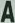
\includegraphics{figures/0020.png}
    \caption{Caracter înainte de aplicarea rotației}
  \end{subfigure}
  \hfill
  \begin{subfigure}[b]{0.45\textwidth}
    \centering
    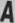
\includegraphics{figures/0020_aug_rot_n05.png}
    \caption{Caracter după aplicarea rotației}
  \end{subfigure}
  \caption{Paralelă între un caracter înainte și după transformare}
  \label{fig:paralela_augmentare}
\end{figure}

Variantele augmentate sunt salvate alături de originale, marcate printr-un sufix dedicat (\texttt{\_aug\_rot}), ceea ce permite distingerea ulterioară a mostrelor sintetice de cele reale. Prin multiplicarea cu factorul de cinci, setul de antrenare crește de la $1862$ la $9310$ mostre.

\subsubsection{Setul de date rezultat}
\indent\par
Prin consolidarea setului de caractere etichetate manual, cu sursa externă de date, a rezultat configurația finală a corpusului de antrenare. Frecvența de apariție a fiecărei clase în cadrul setului final este ilustrată în Figura~\ref{fig:distributia_caracterelor}.

\begin{figure}[H]
  \centering
  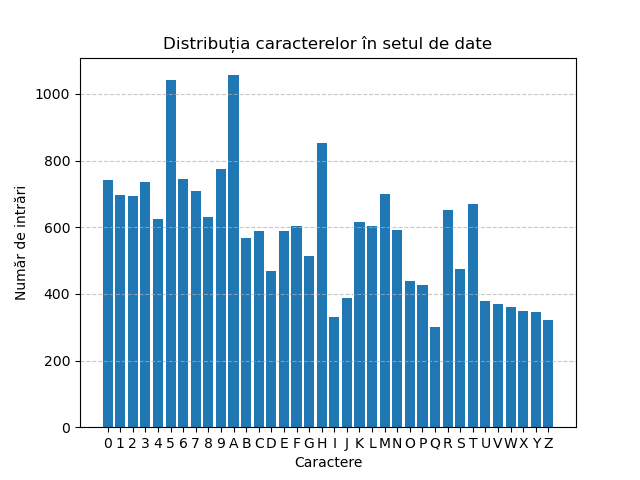
\includegraphics[width=\textwidth]{figures/set_date_plot.png}
  \caption{Distribuția caracterelor în setul de date final}
  \label{fig:distributia_caracterelor}
\end{figure}

\section{Testare și metrici}
\indent\par
Evaluarea sistemului urmărește două niveluri complementare: performanța componentei de recunoaștere a caracterelor, considerată izolat, și performanța întregului lanț de procesare, măsurată de la imaginea de intrare până la șirul de caractere recunoscut.


\subsection{Performanța componentei de recunoaștere a caracterelor}
\indent\par
Pentru evaluarea clasificatorului de caractere, setul de date este împărțit într-un subset de antrenare și unul de testare, în proporție de $80\%$, respectiv $20\%$. Împărțirea este stratificată, astfel încât distribuția claselor să fie păstrată în ambele subseturi.

Metricile raportate pentru clasificator sunt acuratețea globală și raportul de clasificare, care cuprinde, pentru fiecare clasă, precizia (\textit{precision}), rapelul (\textit{recall}) și scorul $F_1$. Aceste metrici sunt completate de matricea de confuzie, utilă pentru identificarea perechilor de caractere frecvent confundate (de exemplu cifra \texttt{0} și litera \texttt{O}, sau cifra \texttt{1} și litera \texttt{I}).

În urma antrenării clasificatorului statistic asupra setului de date menționat anterior au fost obținute următoarele rezultate generale pe subsetul de testare format din 4192 intrări:
\begin{itemize}
  \item \textbf{Acuratețe globală:} 96\%,
  \item \textbf{Precizie medie:} 96\%,
  \item \textbf{Rapel (\textit{Macro Recall}):} 95\%,
  \item \textbf{Scor mediu F1:} 96\%
\end{itemize}

Apropierea dintre valorile medii macro și acuratețea globală indică o performanță uniformă pe ansamblul claselor, fără simboluri defavorizate. Acest comportament este așteptat, întrucât setul combinat menține un volum suficient de exemplare pentru majoritatea claselor, evitând dezechilibrele. În ansamblu, o acuratețe de $96\%$ confirmă că reprezentarea liniarizată a imaginii, combinată cu nucleul RBF (\textit{Radial Basis Function} - Funcție de bază radială), captează suficientă informație distinctivă pentru separarea celor $36$ de clase.

Structura matricei de confuzie poate fi observată în figura~\ref{fig:matrice_confuzie}. Erorile sunt rare și concentrate într-un număr restrâns de perechi de simboluri. Deși rare, erorile persistă în urma procesului de antrenare, în mod special la perechile de caractere care prezintă o similitudine a formei geometrice: pentru perechea formată din cifra \texttt{0} și litera \texttt{O} există 14 erori care apar în mod simetric. De asemenea, există confuzii pentru următoarele perechi: litera \texttt{G} și \texttt{C}, cifra \texttt{1} și litera \texttt{I} sau \texttt{T}.

Aceste confuzii nu au, însă, o pondere uniformă în contextul aplicației. Confuziile de tip cifră-literă, precum \texttt{0}-\texttt{O} sau \texttt{1}-\texttt{I}, sunt în principiu recuperabile: poziția unui simbol în cadrul numărului de înmatriculare determină, conform formatului, dacă acesta trebuie să fie o cifră sau o literă, astfel încât o etapă ulterioară de decodare de format poate valorifica această cunoștință apriori pentru a le clarifica. În schimb, confuziile de tip literă-literă (\texttt{G}-\texttt{C}, \texttt{I}--\texttt{T}) rămân nerezolvabile și constituie limita erorilor clasificatorului.

\begin{figure}[H]
  \centering
  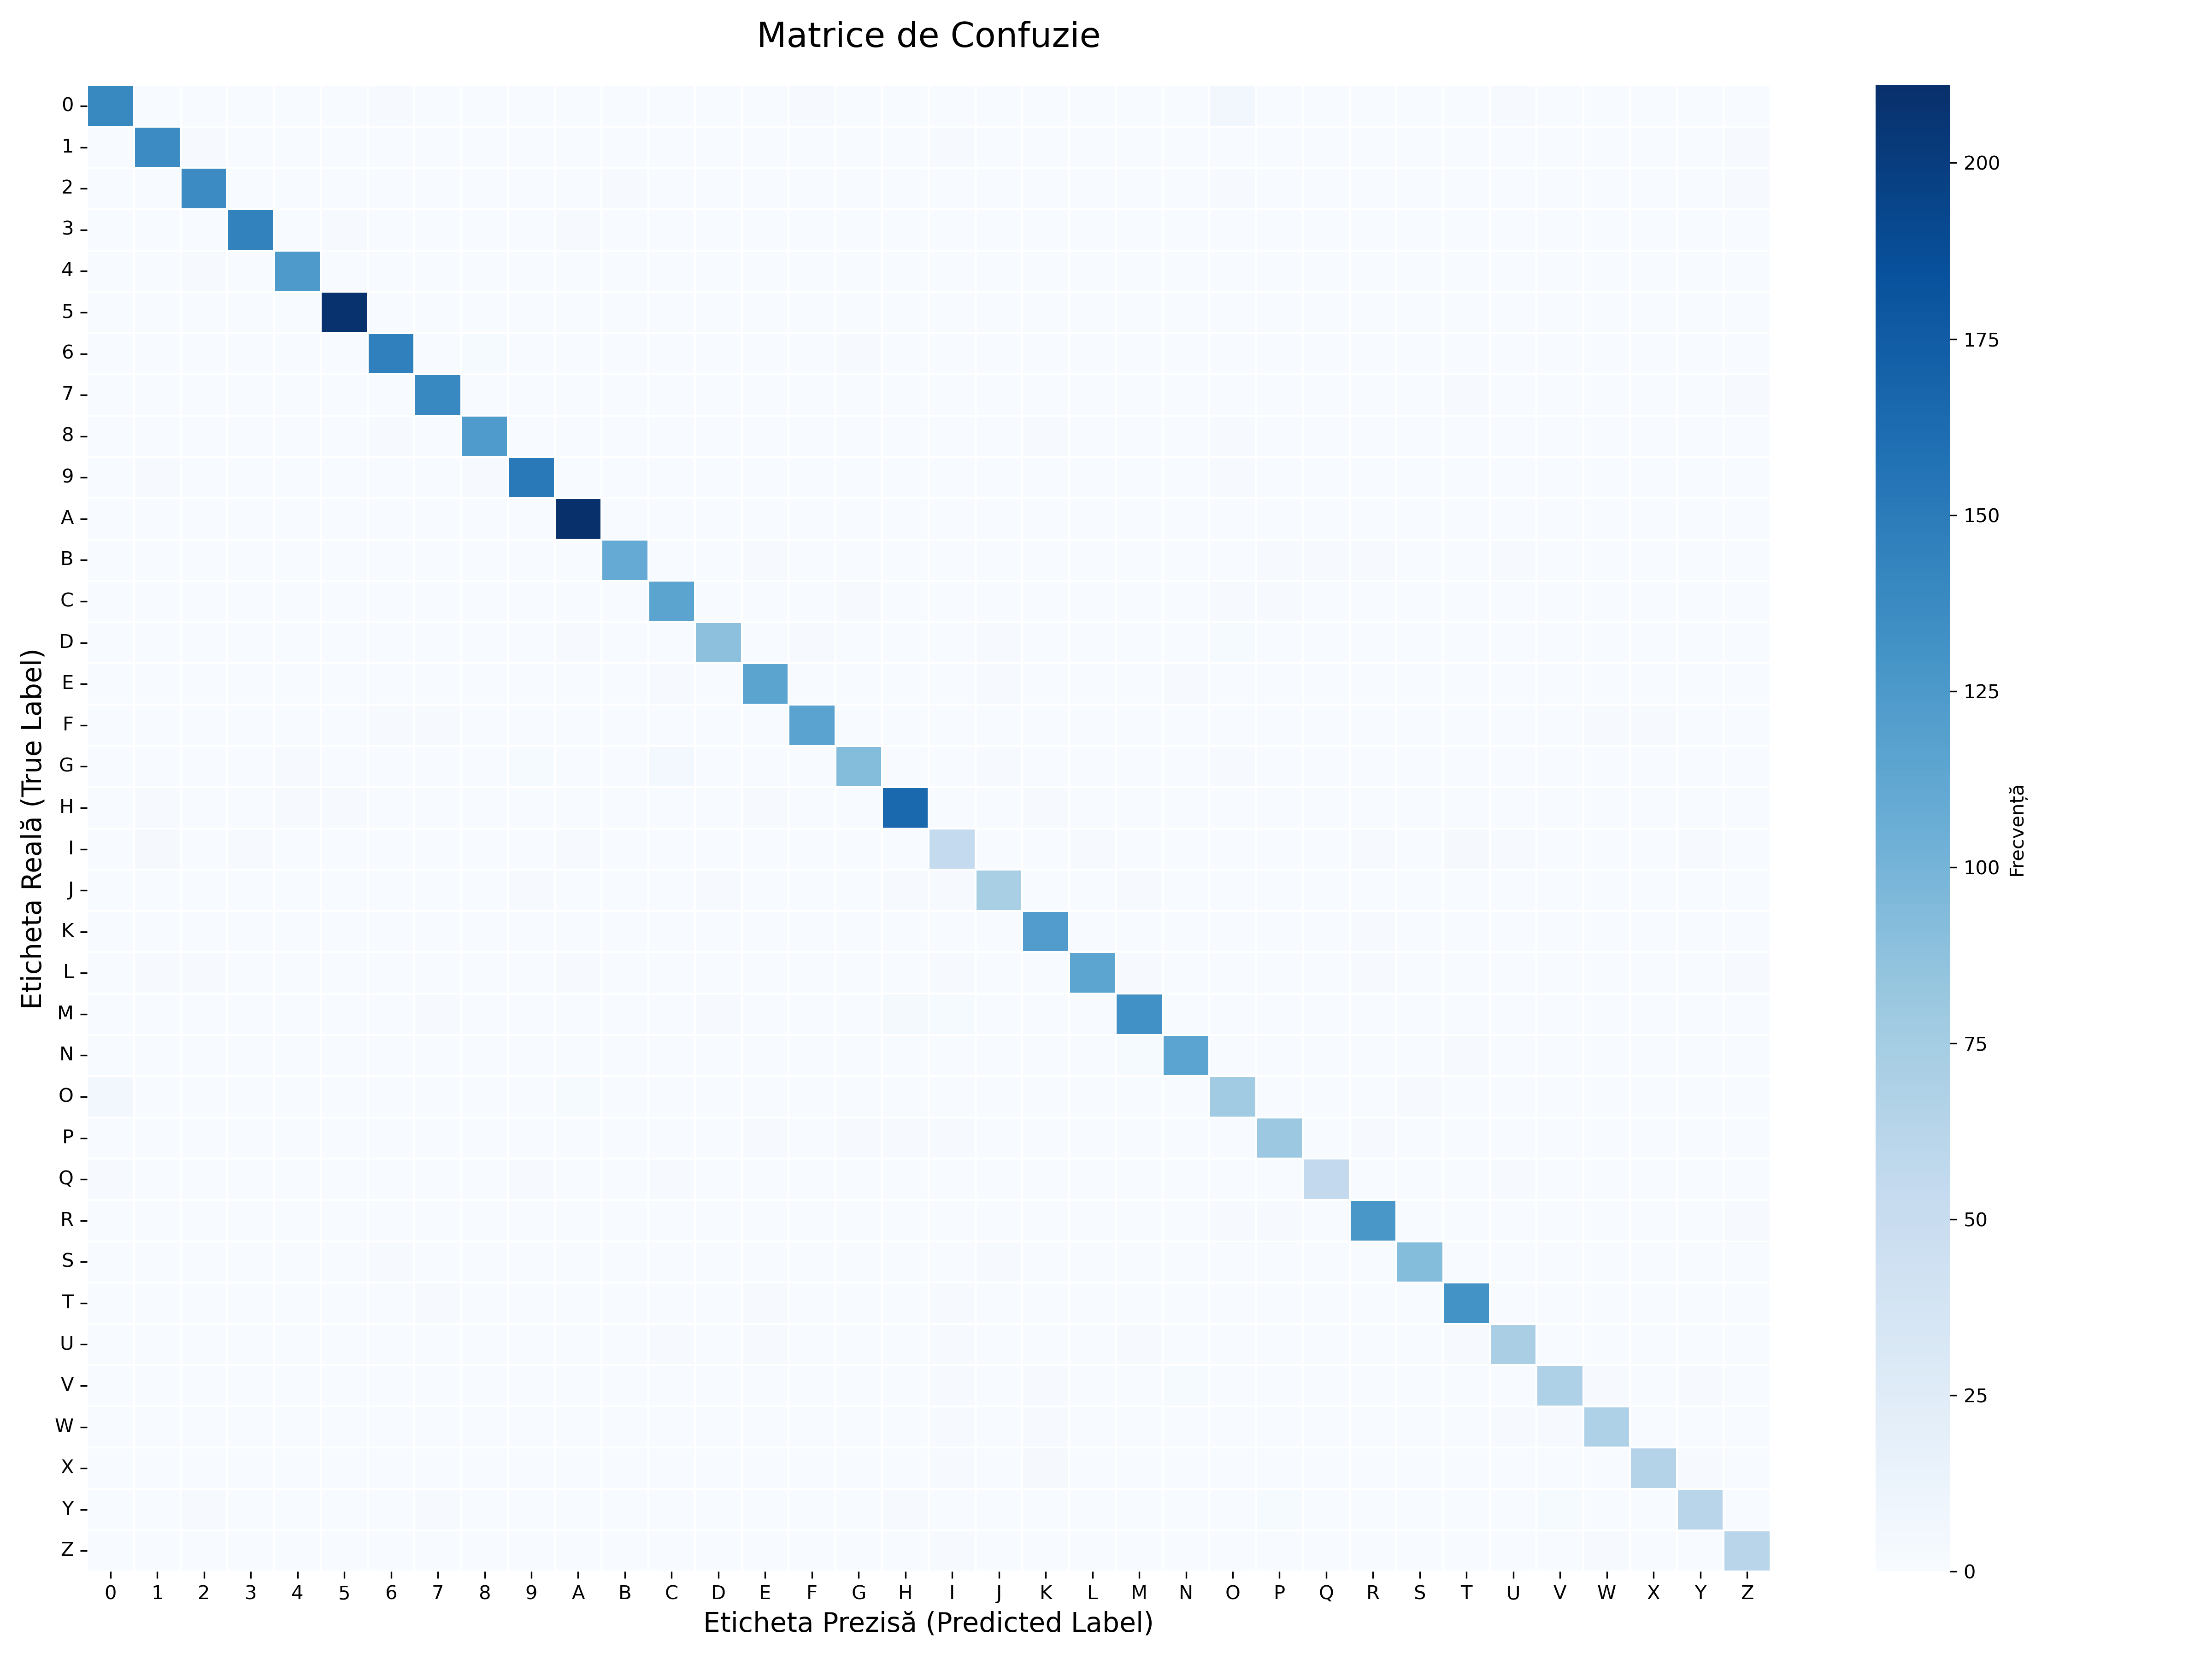
\includegraphics[width=\textwidth]{figures/matrice_confuzie.png}
  \caption{Matricea de confuzie obținută în urma antrenării clasificatorului}
  \label{fig:matrice_confuzie}
\end{figure}

\subsection{Performanța întregului sistem}
\indent\par
Pe lângă evaluarea izolată a clasificatorului, sistemul este evaluat și la nivel de etapă: rata de localizare corectă a plăcuței, rata de segmentare corectă a caracterelor și, în final, metrica integrată (\textit{end-to-end}), reprezentată de proporția plăcuțelor citite corect în întregime. Această din urmă metrică reflectă cel mai fidel performanța percepută a sistemului, întrucât o singură eroare la nivel de caracter invalidează întregul rezultat.

Înainte de a continua cu detaliile tehnice și numerice ale metricilor, este necesară clarificarea metodologiei de evaluare. După cum am menționat în cadrul secțiunii dedicate seturilor de date, colecția destinată evaluării sistemului cuprinde două componente: una internațională, formată din numere de înmatriculare din Thailanda, și una locală, cu numere din România. Astfel, pentru a obține rezultate fidele asupra performanței, utilitarul software \path{src/tools/evaluate.py} a fost rulat în mod separat asupra celor două componente.

Rularea separată a fost necesară și pentru că modulul de recunoaștere a caracterelor a fost adaptat să valorifice o cunoștință apriori esențială: structura formatului numărului de înmatriculare. Întrucât poziția fiecărui simbol determină, conform formatului regional, dacă acesta trebuie să fie cifră sau literă, metoda \texttt{predict} a clasei \texttt{CharacterRecognition} înlocuiește predicția top-1 a SVM-ului cu marginile furnizate de \texttt{decision\_function} și restrânge subsetul de clase admis de format. Această decodare condiționată recuperează tocmai confuziile de tip cifră-literă discutate anterior (\texttt{0}-\texttt{O}, \texttt{1}-\texttt{I}), care altfel ar invalida întregul șir.

\subsubsection{Evaluarea localizării corectă a plăcuței}
\indent\par
Pentru a putea cuantifica proporția în care sistemul extrage în mod corect regiunea de interes ce conține numărul de înmatriculare, a fost folosită metrica \textit{Intersecție supra Reuniune} (IoU - \textit{Intersection over Union}). Pentru a calcula această metrică, este nevoie atât de regiunile delimitate de sistem drept zone candidate, cât și de coordonatele reale ale plăcuței (regiunea adnotată manual).

Deoarece modulul de localizare propune mai multe regiuni candidat pentru o singură imagine, evaluarea performanței se face doar raportat la zona cu cel mai mare raport IOU. Astfel, o imagine pentru care există cinci predicții posibile pentru regiunea de interes, va fi redusă la un singur rezultat IOU. Această abordare a fost aleasă deoarece, precum am menționat în capitolul anterior, modulul de segmentare extrage implicit zona ideală, mai exact zona cu cel mai mare IOU.

În urma rulării celor două utilitare software, \path{src/tools/evaluate.py} și \path{src/tools/metrics.py}, modulul de localizare obține un IoU mediu de $\approx0.65$ pe componenta internațională și $\approx0.63$ pe cea locală. Valorile moderate se explică prin natura modulului de extracție: etapele de dilatare orizontală și de fuziune a candidaților extind în mod deliberat regiunea propusă, pentru a garanta că plăcuța nu este fragmentată și că toate caracterele rămân în interiorul zonei de interes. Deoarece metrica IoU penalizează în egală măsură surplusul și deficitul de suprafață, o margine de câțiva pixeli în jurul plăcuței reduce sensibil scorul, chiar și atunci când localizarea este corectă din punct de vedere funcțional. Această explicație este confirmată practic de creșterea scorului IoU la $\approx0.80$ în momentul introducerii unei etape de validare cu un prag minim de încredere de $0.50$.

\subsubsection{Evaluarea segmentării caracterelor}
\indent\par
Spre deosebire de localizare, pentru care există o adnotare manuală a regiunii de interes, etapa de segmentare nu dispune de o delimitare de referință a fiecărui caracter în parte. Din acest motiv, evaluarea segmentării se realizează indirect, prin compararea numărului de caractere extrase de sistem cu lungimea șirului de referință al plăcuței. Metrica adoptată este acordul la nivel de număr de caractere: pentru fiecare imagine, raportul dintre minimul și maximul celor două valori, după cum este prezentat în Ecuația \ref{eq:acord_caractere}.

\begin{equation}
    \text{Acord} = \frac{\min(n_{\text{seg}}, n_{\text{gt}})}{\max(n_{\text{seg}}, n_{\text{gt}})}
    \label{eq:acord_caractere}
\end{equation}

\noindent unde $n_{\text{seg}}$ este numărul de caractere segmentate, iar $n_{\text{gt}}$ este numărul de simboluri din adevărul de referință. Valoarea $1$ indică un acord perfect, iar abaterile, fie prin sub-segmentare, fie prin supra-segmentare reduc proporțional scorul. Această metrică surprinde corectitudinea structurală a segmentării fără a presupune o adnotare la nivel de caracter.

Pentru componenta internațională, etapa de segmentare a obținut un acord mediu de $\approx0.85$, iar pentru cea locală de $\approx0.82$. Interpretarea acestor valori sugerează că, în mare parte, modulul de segmentare extrage un număr apropiat de caractere relativ la sursa de adevăr. Diferența rămasă până la acordul perfect este atribuibilă, pe de o parte, plăcuțelor pentru care etapa de localizare a furnizat un decupaj imperfect, iar pe de altă parte cazurilor de fuziune a caracterelor adiacente sau de fragmentare a caracterelor cu structură discontinuă.

\subsubsection{Evaluare E2E}
\indent\par
Metrica integrată (\textit{end-to-end}) reflectă cel mai fidel performanța percepută a sistemului, întrucât consideră corectă o plăcuță doar atunci când întregul șir de caractere coincide cu adevărul de referință. O singură eroare la nivel de caracter, indiferent de poziția sa, invalidează rezultatul. Pentru a completa această măsură binară, evaluarea raportează și \emph{similaritatea Levenshtein} a șirului recunoscut față de cel de referință, o metrică mai fină care surprinde gradul de corectitudine parțială a predicțiilor invalidate.

Evaluarea pe componenta internațională a setului de date a indicat o acuratețe de $\approx0{,}69$, în timp ce pentru componenta națională s-a obținut un procentaj de $\approx0{,}73$. Similaritatea Levenshtein medie depășește în ambele cazuri pragul de $\approx0{,}80$. Această valoare, semnificativ mai ridicată decât rata de potrivire exactă, confirmă faptul că o proporție importantă a predicțiilor invalidate diferă de adevărul de referință printr-un singur caracter. Cel mai adesea, aceste erori punctuale sunt cauzate de posibilele confuzii vizuale ale modulului de recunoaștere, sau diferitele artefacte vizuale prezente pe o plăcuță, evidențiate în Figura~\ref{fig:artefacte}

\begin{figure}[H]
  \centering
  \begin{subfigure}[b]{0.48\textwidth}
    \centering
    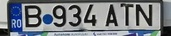
\includegraphics[width=\textwidth]{figures/B934ATN.png_lp_1.jpg}
    \caption{Bulină albastră care va fi segmentată în mod incorect drept un caracter}
  \end{subfigure}
  \hfill
  \begin{subfigure}[b]{0.48\textwidth}
    \centering
    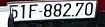
\includegraphics[width=\textwidth]{figures/CarLongPlate60_jpg.rf.9ac70cfc36770f5233142a727c52d534.jpg_lp_0.jpg}
    \caption{Artefact care blochează parțial numărul de înmatriculare}
  \end{subfigure}
  \caption{Exemple de artefacte ce pot deteriora procesul de recunoaștere}
  \label{fig:artefacte}
\end{figure}

\section{Experimente}
\indent\par
Experimentele prezentate în această secțiune urmăresc să justifice, prin rezultate cantitative, deciziile de proiectare adoptate în fluxul de procesare și să evidențieze contribuția fiecărei componente la performanța de ansamblu. Ele sunt organizate în trei părți: comparația dintre două abordări ale etapei de localizare, comparația dintre cele două abordări ale etapei de segmentare și seria de îmbunătățiri progresive aduse fluxului de recunoaștere.

\subsection{Comparația abordărilor de localizare}
\indent\par
Înainte de adoptarea abordării bazate pe operatorul Sobel și pe operațiile morfologice descrise anterior, etapa de localizare a fost implementată într-o manieră similară, dar cu un discriminant principal al regiunilor complet diferit: varianta inițială se baza pe aproximarea poligonală a contururilor.

Lanțul de preprocesare urma aceiași pași ca varianta curentă: conversia în tonuri de gri a cadrului primit de la modulul de intrare, atenuarea zgomotului și binarizarea, cu două deosebiri: reducerea zgomotului se realiza printr-un operator diferit de filtrul median, iar accentuarea muchiilor folosea detectorul de contururi Canny în locul operatorului Sobel. Extragerea contururilor (\texttt{findContours}) era identică cu cea din varianta curentă, însă selecția primilor \texttt{top\_k} candidați se făcea pe baza aproximării poligonale (\texttt{approxPolyDP}). Acest discriminant s-a dovedit însă nefiabil: în practică, multe dintre plăcuțe erau extrase ca poligoane cu un număr ridicat de laturi, ratând astfel criteriul geometric al formei dreptunghiulare. Tabelul~\ref{tab:cmp-localizare} sintetizează diferența de performanță dintre cele două abordări.

\begin{table}[H]
  \centering
  \begin{tabular}{lc}
    \hline
    Metodă de localizare & IoU mediu \\
    \hline
    Aproximare poligonală (\texttt{approxPolyDP}, variantă explorată) & $< 0{,}40$ \\
    Sobel + morfologie + \texttt{top\_k} (abordarea propusă) & $\approx0{,}60$ \\
    \hline
  \end{tabular}
  \caption{Comparație între cele două abordări ale etapei de localizare, evaluate prin același lanț de selecție \texttt{top\_k} și corecție de înclinare.}
  \label{tab:cmp-localizare}
\end{table}

Abordarea bazată pe aproximare poligonală nu a reușit să depășească un IoU mediu de $0{,}40$, în timp ce abordarea curentă atinge aproximativ $0{,}60$. Cauza principală a limitării este dependența de detectarea unui contur închis și dreptunghiular al marginii plăcuței: în condiții reale, această margine este frecvent fragmentată, astfel încât aproximarea poligonală fie nu produce un patrulater, fie îl produce deplasat față de plăcuța reală. Spre deosebire de aceasta, abordarea bazată pe Sobel și operații morfologice nu depinde de conturul marginii plăcuței, ci de concentrarea de muchii verticale generate de caractere: un semnal mai robust și independent de calitatea conturului exterior.

\subsection{Comparația abordărilor de segmentare}
\indent\par
Pentru etapa de segmentare au fost considerate două dintre abordările prezentate în capitolul~\ref{chap:segmentare}: segmentarea bazată pe proiecții orizontale și verticale și cea bazată pe contururi, ghidată de cunoștințe apriori privind aspectul caracterelor. Înainte de detalierea tehnică a celor două, tabelul~\ref{tab:cmp-segmentare} sintetizează diferența de performanță dintre ele, diferență care a fundamentat alegerea abordării pe contururi.

\indent\par
\begin{table}[H]
  \centering
  \begin{tabular}{lccc}
    \hline
    Metodă de segmentare & Localizare & Segmentare & End-to-end \\
    \hline
    Bazată pe proiecții (variantă explorată) & 0{,}65 & 0{,}20 & 0{,}05 \\
    Bazată pe contururi (implementarea propusă) & 0{,}65 & 0{,}85 & 0{,}69 \\
    \hline
  \end{tabular}
  \caption{Comparație directă între cele două abordări ale etapei de segmentare, pe același set de candidați produși de etapa de localizare.}
  \label{tab:cmp-segmentare}
\end{table}

Aceste diferențe uriașe nu provin dintr-un avantaj al setului care să favoritizeze metodele bazate pe contururi, ci din modul în care fiecare abordare tratează semnalul.

Analiza proiecțiilor comprimă imaginea binară într-un profil unidimensional, obținut prin însumarea pixelilor de prim-plan pe coloane, iar separarea caracterelor depinde de existența unor văi suficient de adânci între vârfurile asociate fiecărui simbol. Pe plăcuțele din setul de evaluare, această condiție este rar îndeplinită: reziduurile cadrului (banda UE, șuruburile de prindere) și, mai ales, înclinarea de câteva grade a plăcuței determină suprapunerea pe verticală a coloanelor caracterelor adiacente, astfel încât văile dintre ele nu mai coboară sub pragul de extragere a vârfurilor.

Abordarea bazată pe contururi nu este afectată de acest fenomen, întrucât decide la nivelul fiecărei componente conexe în parte, izolând fiecare caracter prin propriul contur închis, independent de unghiul de înclinare și de spațierea dintre simboluri.

\subsection{Îmbunătățiri progresive ale fluxului de recunoaștere}\label{sec:imbunatatiri}
\indent\par
Plecând de la configurația de bază descrisă în secțiunile anterioare, au fost adoptate, succesiv, cinci intervenții incrementale care vizează etapele de segmentare, decodare și clasificare. Evaluarea s-a făcut pe setul de date dedicat evaluării sistemului, iar metricile raportate sunt rata \textit{end-to-end} (egalitate exactă), similaritatea Levenshtein a OCR-ului, acordul la nivel de număr de caractere segmentate și IoU-ul localizării. Tabelul~\ref{tab:imbunatatiri} sintetizează contribuția cumulativă a fiecărei intervenții.

\begin{table}[H]
  \centering
  \small
  \begin{tabular}{p{6.2cm}cccc}
    \hline
    Configurație & End-to-end & OCR sim. & Acord seg. & IoU \\
    \hline
    Bază & 0{,}489 & 0{,}768 & 0{,}809 & 0{,}588 \\
    \quad + reconstrucția segmentării  & 0{,}597 & 0{,}801 & 0{,}839 & 0{,}588 \\
    \quad + decodare condiționată de format & 0{,}645 & 0{,}801 & 0{,}839 & 0{,}588 \\
    \quad + trăsături HOG pentru SVM & 0{,}667 & 0{,}807 & 0{,}839 & 0{,}588 \\
    \quad + pre-procesare cu conservarea proporțiilor & 0{,}677 & 0{,}806 & 0{,}839 & 0{,}588 \\
    \quad + padding LP și augmentare cu rotații & \textbf{0{,}694} & 0{,}813 & 0{,}843 & 0{,}589 \\
    \hline
  \end{tabular}
  \caption{Contribuția cumulativă a celor cinci intervenții. Fiecare linie include modificările liniilor anterioare. Cumulat, rata end-to-end a crescut cu $20{,}5$ puncte procentuale ($91 \to 129$ plăcuțe corecte din $186$).}
  \label{tab:imbunatatiri}
\end{table}

\subsubsection{Reconstrucția etapei de segmentare}
\indent\par
Înainte de intervenție, decupajul de plăcuță era binarizat direct, iar contururile externe erau filtrate exclusiv prin raportul de aspect $w/h$, cu un prag inferior de $0{,}15$. Matricea de confuzii a arătat două surse sistematice de erori: aproximativ $250$ de caractere lipsă (dominate de $5\to\emptyset$ cu $55$ de cazuri, $1\to\emptyset$ cu $48$ de cazuri) și aproximativ $30$ de caractere inserate fals ($\emptyset\to A$, $\emptyset\to T$, $\emptyset\to H$). Caracterul \texttt{1}, cu un raport real $w/h$ între $0{,}07$ și $0{,}12$, era respins în întregime de pragul geometric, iar reziduurile cadrului plăcuței (banda UE, șuruburile de prindere) produceau contururi care imitau caractere reale.

Soluția a constat în (1) restrângerea decupajului la cea mai mare componentă conexă deschisă din interiorul plăcuței, eliminând cadrul înainte de binarizare; (2) coborârea pragului $w/h$ la $0{,}08$, recuperând caracterul \texttt{1}; (3) respingerea contururilor care ating marginile laterale ale plăcuței tăiate, anulând patternul de inserții; (4) o trecere de consistență pe înălțimi, care elimină casetele aflate în afara intervalului $[0{,}55\,m, 1{,}45\,m]$, unde $m$ este înălțimea mediană a supraviețuitorilor; (5) un divizor de blocuri largi care, pentru casete cu $w > 1{,}2\,h$, taie la coloana cu cea mai joasă proiecție verticală, recuperând caracterele lipite. Inserțiile au scăzut de la $\sim 30$ la $\sim 5$, iar rata end-to-end a urcat cu $10{,}8$ puncte procentuale.

Au fost respinse explicit aplicarea unei închideri morfologice $3\times3$, care, pe plăcuțe de $\sim 27$ de pixeli înălțime, a unit caracterele adiacente (numărul de contururi crude a scăzut de la $23$ la $4$ într-un caz observat), și varianta verticală $(2,1)$, cu același efect în formă atenuată.

\subsubsection{Decodare condiționată de format}
\indent\par
Analiza matricii de confuzie a indicat substituții frecvente între clase vizual similare (\texttt{4}$\to$\texttt{F}, \texttt{O}$\to$\texttt{0}, \texttt{1}$\to$\texttt{I}), generate de ambiguitatea internă a SVM-ului. Indiferent de regiune, structura numărului de înmatriculare oferă tocmai acest context: formatul fixează, pentru fiecare poziție, dacă simbolul așteptat este o cifră sau o literă. Cunoștințele pre-existente asupra formatului pot facilita procesul de clasificare, restrângând domeniul de predicții posibile.

Modificarea, localizată în metoda \texttt{predict} a clasei \texttt{CharacterRecognition}, este formulată independent de un format anume. Ea înlocuiește predicția top-1 a SVM-ului cu marginile furnizate de \texttt{decision\_function} și restrânge și restrânge subsetul de clase admis de format.

Atunci când o lungime dată admite mai multe formate candidate, fiecare șablon este evaluat, iar cel cu marginea medie pe poziție cea mai mare este selectat. Pentru lungimile care nu corespund niciunui format, decodarea revine la varianta neconstrânsă, evitând orice regresie. Aceeași logică se aplică nemodificat atât plăcuțelor românești și thailandeze.

\subsubsection{Trăsături HOG pentru clasificator}
\indent\par
Reprezentarea pe $784$ de dimensiuni (intensitățile brute ale pixelilor $28\times28$) a fost înlocuită cu un descriptor HOG.

Modelul a fost re-antrenat, atingând o acuratețe de $97\%$ pe subsetul independent. În pipeline-ul integrat, rata \textit{end-to-end} a urcat cu $2{,}2$ puncte procentuale (la $66{,}7\%$). Un alt rezultat este scăderea numărului de perechi de erori din matricea de confuzie de la $82$ la $70$, indicând o concentrare a acestora în categorii mai bine definite și mai ușor de abordat în continuare.

\subsubsection{Păstrarea proporțiilor caracterului}
\indent\par
Ultima modificare rezolvă o limitare a etapei de pregătire a caracterului: redimensionarea directă la $28\times28$ deforma raportul de aspect al claselor înguste. Un caracter \texttt{1}, cu $w/h \approx0{,}12$ la segmentare, devenea un pătrat, iar descriptorul HOG raporta o distribuție de orientări similară cu cea a unui \texttt{I}, \texttt{T} sau \texttt{L}. Modificarea din logica funcției \texttt{preprocess\_char} completează imaginea cu o margine constantă până la un pătrat, înainte de redimensionarea la $28\times28$.


\subsubsection{Augmentare cu rotații a setului de antrenare}
\indent\par
Schimbarea descrisă în cele ce urmează are drept scop creșterea robusteții clasificatorului la diferența dintre distribuția setului de antrenare și cea din mediul de execuție. Această ajustare a urcat rata end-to-end cu $1{,}7$ puncte procentuale (la $69{,}4\%$).

Intervenția constă într-un script de augmentare (\texttt{src/augment\_dataset.py}) care, pentru fiecare exemplar etichetat din setul obținut în mod manual, generează patru variante rotite la $\pm 3^\circ$ și $\pm 5^\circ$ în jurul centrului, cu marginea completată prin aceeași metodă \texttt{preprocess\_char}). Setul de antrenament crește astfel de la $1862$ la $9310$ mostre.

\subsubsection{Bilanț}
\indent\par
Cumulat, cele cinci intervenții au urcat rata \textit{end-to-end} de la $48{,}9\%$ la $69{,}4\%$. Două limitări reziduale rămân vizibile: tăierea caracterului inițial al plăcuței, cauzată în etapa de localizare și un set restrâns de substituții vizual ambigue dintre litere sau dintre cifre (\texttt{Y}$\to$\texttt{M}, \texttt{F}$\to$\texttt{6}, \texttt{1}$\to$\texttt{I}).
